%%%%%%%%%%%%%%%%%%%%%%%%
%% Sample use of the infthesis class to prepare a thesis. This can be used as 
%% a template to produce your own thesis.
%%
%% The title, abstract and so on are taken from Martin Reddy's csthesis class
%% documentation.
%%
%% MEF, October 2002
%%%%%%%%%%%%%%%%%%%%%%%%

%%%%
%% Load the class. Put any options that you want here (see the documentation
%% for the list of options). The following are samples for each type of
%% thesis:
%%
%% Note: you can also specify any of the following options:
%%  logo: put a University of Edinburgh logo onto the title page
%%  frontabs: put the abstract onto the title page
%%  deptreport: produce a title page that fits into a Computer Science
%%      departmental cover [not sure if this actually works]
%%  singlespacing, fullspacing, doublespacing: choose line spacing
%%  oneside, twoside: specify a one-sided or two-sided thesis
%%  10pt, 11pt, 12pt: choose a font size
%%  centrechapter, leftchapter, rightchapter: alignment of chapter headings
%%  sansheadings, normalheadings: headings and captions in sans-serif
%%      (default) or in the same font as the rest of the thesis
%%  [no]listsintoc: put list of figures/tables in table of contents (default:
%%      not)
%%  romanprepages, plainprepages: number the preliminary pages with Roman
%%      numerals (default) or consecutively with the rest of the thesis
%%  parskip: don't indent paragraphs, put a blank line between instead
%%  abbrevs: define a list of useful abbreviations (see documentation)
%%  draft: produce a single-spaced, double-sided thesis with narrow margins
%%
%% For a PhD thesis -- you must also specify a research institute:
\documentclass[msc,ai,logo,twoside]{infthesis}

%% For an MPhil thesis -- also needs an institute
% \documentclass[mphil,ianc]{infthesis}

%% MSc by Research, which also needs an institute
% \documentclass[mscres,irr]{infthesis}

%% Taught MSc -- specify a particular degree instead. If none is specified,
%% "MSc in Informatics" is used.
% \documentclass[msc,cogsci]{infthesis}
% \documentclass[msc]{infthesis}  % for the MSc in Informatics

%% Master of Informatics (5 year degree)
% \documentclass[minf]{infthesis}

%% Undergraduate project -- specify the degree course and project type
%% separately
% \documentclass[bsc]{infthesis}
% \course{Artificial Intelligence and Psychology}
% \project{Fourth Year Project Report}

%% Put any \usepackage commands you want to use right here; the following is 
%% an example:
\usepackage{natbib}
\usepackage{tikz}
\usetikzlibrary{shapes,arrows}

%% Information about the title, etc.
\title{Testing a Critique of Computational Cognitive Modelling}
\author{Arnaud Henry}
\shieldtype{4} %% coloured logo

%% If the year of submission is not the current year, uncomment this line and 
%% specify it here:
% \submityear{1785}

%% Optionally, specify the graduation month and year:
% \graduationdate{February 1786}

% Every figure will be centered
\makeatletter
\g@addto@macro\@floatboxreset\centering
\makeatother

%% Specify the abstract here.
\abstract{%
    This doctoral thesis will present the results of my work into the
    reanimation of lifeless human tissues.
}

%% Now we start with the actual document.
\begin{document}

%% First, the preliminary pages
\begin{preliminary}

%% This creates the title page
\maketitle

%% Acknowledgements
\begin{acknowledgements}
I would like to thanks my awesome flatmates, including the dog, the ghosts and the mice.
\end{acknowledgements}

%% Next we need to have the declaration.
\standarddeclaration

%% Finally, a dedication (this is optional -- uncomment the following line if
%% you want one).
% \dedication{To my mummy.}

%% Create the table of contents
\tableofcontents

%% If you want a list of figures or tables, uncomment the appropriate line(s)
% \listoffigures
% \listoftables

\end{preliminary}


\tikzstyle{layer}=[draw,rectangle,minimum width=5cm, minimum height=0.7cm, align=center]
\tikzstyle{component}=[draw, circle, align=center, minimum height=2cm]

%%%%%%%%
%% Include your chapter files here. See the sample chapter file for the basic
%% format.


\chapter{Introduction}

% what is the problem ?
Speech recognition is the act of correctly assigning lexical items to an acoustic speech signal.
Doing so in an automated way has proven to be a considerable challenge. Although the task seems somehow trivial as we communicate effortlessly with others around us, there are many difficulties arising when one attempts to build a computational model as efficient as we are.

First, each spoken word is composed of speech sounds that are influenced by one another. 
% TODO example of coarticulation
For example

Secondly, spoken words in a sentence are not usually separated by silence. This means that word boundaries have to be guessed by the model - a problem a written text recogniser does not have to deal with, as written words are separated by blanks.
%TODO cite (taken from McClelland86) :
% there are some cues in the speech stream, but as several investigators have pointed out (Cole & Jakimik, 1980; Grosjean & Gee, 1984; Thompson, 1984), they are not always sufficient,
Finally, we often communicate in noisy environments, and each speaker has its own accent and way of pronouncing, not to mention that the intonation of the same utterance by a single speaker changes depending on his mood.

All these facts are a reason as to why no computational model has managed to match our ability to recognise speech. 

% why is it important ?

An approach to solving the problem of automatic speech recognition is the development of computational cognitive models, in which much attention is draw to the cognitive processes involved in speech recognition. These models aim at reproducing empirical data collected through diverse experiments made on human subjects. 


% talk about TRACE

% briefly mention the abstract / concrete universal stuff
% present what the paper is about


\section{Overview}
% overview of the rest of the paper



\chapter{Background}

% If you want to mention the Cohort model: biggest pb is that it doesn't allow noise

\section{The TRACE model}

James McClelland and Jeffery Elman first developed a model of phoneme identification from real speech called TRACE I \citep{elman1986exploiting}. The model had adjustable feature to phoneme connection strengths in order to deal with variability due to local phonetic context. It could extract features from real speech and correctly identify 90\% of stop consonants from monosyllable inputs.
Because dealing with real speech involved getting concerned with exact duration of different features and phonemes in different contexts, it was harder to focus on the psychological aspect of the model and thus was not extendible in that form. This is why the authors developed another model, TRACE II, in which input to the model was mock speech, but where a lexical layer of processing could be added, enabling to account for a large amount of available psychological data. This is the model we are interested in and which is simply referred to TRACE in the literature.


\subsection{Motivations}

The interactive activation architecture of the TRACE model, which we will describe in detail in the next section, is motivated by several aspects of speech that have been discussed by Klatt \citep{klatt1979speech} and which McClelland and Elman refer to in their seminal paper:

\begin{itemize}
\item Speech is spread across time. This fact implies that a model of speech recognition has to keep a record of previous utterances in order to process incoming input. Not only previous context, but it has been shown that also subsequent context has an influence on perception at a specific time \citep{salasoo1985interaction} \citep{thompson1984word}. This means that a successful model cannot have static phoneme or word recognition, in the sense that it must be possible to alter the perception of previously recognised entities.

\item Speech units overlap. Whether at the word or phoneme level, there are no reliable cues as to where units are separated. Indeed, words in fast speech - that is, conversational speech - tend to run into one other, sometimes sharing a phonetic sound in order to make the pronunciation easier for the speaker. In a similar way, phonemes overlap in such a way that it is impossible to tell at which point in time each phoneme starts and ends. In contrast to these two observations, written text has an advantage as letters are clearly distinguishable and words are separated by white spaces. The fact that speech units overlap means that phoneme and word recognition doesn't rely on precise segmentation of the input.

\item Speech units are context-sensitive. The way phonemes are pronounced depends greatly on surrounding phonemes. For example, %TODO coarticulation example

This effect known as coarticulation has caused many problems to cognitive modellers. McClelland and Elman take it into account by allowing connections to alter depending on the context.

\item Speech is perceived in noise. We often converse rather efficiently in noisy environments, 
and this fact alone implies that a model of speech recognition must not rely on the accurate recognition of any part of the speech.

\end{itemize}

Most of these facts are peculiar to speech and make the general task of speech recognition more difficult than written text recognition. 



\subsection{Architecture}
%% presentation of the TRACE model

The TRACE model is composed of three layers of processing: features, phonemes and words, in which every unit is replicated across time.
 
At the feature level, a set of seven dimensions is used to represent mock speech: Consonantal, Vocalic, Diffuseness, Acuteness, Voicing, Power and Burst. The first five were taken from the famous work of \citep{jakobson1961preliminaries}, Power was included to differentiate further vowels from consonants, and Burst was introduced to help discriminate among the different stop consonants. 
%These features could be extracted from real speech with relative success as the authors had done in TRACE I, however, as been mentioned before, the purpose of the TRACE II model is to provide greater insight into the cognitive processes involved in speech recognition, and dealing with low-level details is an obstacle to that goal.
Each of the seven dimensions is divided into nine value ranges, eight of which correspond to a grade from low to high. The ninth value is reserved to represent silence, and thus is used only by the silence phoneme "-". The 63 (7*9) units are replicated for each of the 25ms time slices of the model, and are filled in progressively by values corresponding to the input of the model. Figure \ref{TRACEarch} shows an example of a complete filling for three of the seven features for the input \textit{tea cup}.

%TODO diagram of the model
\begin{figure}
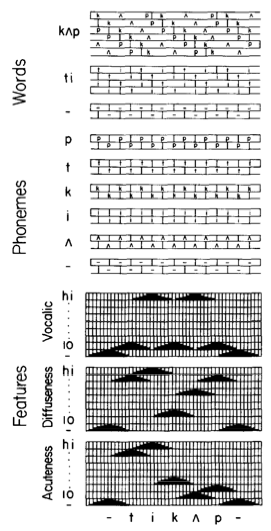
\includegraphics[height=13cm]{images/TRACE_architecture.png}
\caption{A subset of the units in TRACE. Each rectangle represents a different unit at each level. The input feature specifications for the phrase ”tea cup” are indicated for the three following dimensions: Acuteness, Diffuseness and Vocalic. \citep{mcclelland1986trace}}
\label{TRACEarch}
\end{figure}

At the phoneme level, 15 phonemes are represented by units spanning 6 time slices and replicated every 3 time slices, as can be seen in figure \ref{TRACEarch} for a few phonemes. Note that this means adjacent phoneme units overlap, just as it is observed in real speech. Each phoneme unit receives activation from the feature units that make up that phoneme. McClelland and Elman came up with feature specifications for the following 14 phonemes: /b/, /p/, /d/, /t/, /g/, /k/ (stop consonants), /s/, /S/ (fricatives), /l/, /r/ (liquids), /a/, /i/, /u/ and /\^/ (vowels), and also added a silence phoneme /-/. There are inhibitory connections between units representing different phonemes which overlap in time, such that if a certain phoneme at a certain time slice receives activation from the feature level, it will inhibit other phonemes units at that time slices and three time slices apart (since a phoneme unit spans 6 time slices).

At the word level, each word is represented by units replicated every 3 time slices (as for the phonemes). The time span of these units depend on the length of the word, 6 time slices being allocated to each phoneme which compose that word (referring to the example in figure \ref{TRACEarch}, /k\^p/ spans 18 time slices and /ti/ spans 12 time slices). Word units receive activation from the phoneme units that match and are aligned with the particular phonemes that make up the word. For example, the phoneme /t/ at time slice 6 will activate all word units starting at that time with /t/ being their first phoneme, and also all words units starting at time slice 0 which have /t/ in second position. As for the phoneme level, word units inhibit one another if they represent a different word and are overlapping in time. This is the basis of the interactive activation mechanism present in TRACE.

In addition to the excitatory bottom-up connections between layers and intra-layer inhibitory connections, TRACE provides top-down excitatory connections from words to phonemes. Each phoneme unit can therefore receive activation from words which contain that phoneme at that particular time slice.




% words




% how a typical run goes?


\subsection{Advantages}
% what phenomena it accounts for

\subsection{Limitations}
% limitations:
% - not physiologically plausible
% - hardwired; cannot learn
% - not expandable to the full english phoneme set and bigger lexicon (=> other languages as well)



\section{Evolution of cognitive modelling}
% Evolution of the model (not much evolution...)
\citep{chawlaShillcock}


\chapter{Methodology}



\section{Philosophical critique}


%% Philosophical critique
% Abstract and Concrete universals (cite Shillcock)
% Simplicity vs Completeness
% Ziegler: nested... (augmenting the model)
% A model should escape from the full complexity of the world, but also be able to relate, "come back" to it.
% Ahissar & Hochstein: magnocellular pathways (some fast pathways draw a sketch of the input and comes back down to meet the 

\section{}
%% Changes brought to the model

% Extended phoneme set
% Extended lexicon

% talk about the interface built to help evaluate the performance of the model comparatively to the original (+screenshot, in appendix maybe)
% The parameters [decay, rest, weights] are unmodified


Check out figure \ref{modified}


\begin{figure}[!h]
\begin{tikzpicture}[scale=1]

% node definitions
 \foreach \place/\name in {{(0,0)/features}, {(0,2)/phonemes}, {(0,4)/words}}
    \node[layer] (\name) at \place {\name};
\node[component] (schwa) at (6,2){schwa};
\node[component] (lex) at (8,4){lexical\\stress};

% arrows
  \foreach \source/\dest in {features/phonemes, phonemes/words, words/phonemes, features/schwa, schwa/phonemes, schwa/words, schwa/lex, lex/schwa}
    \path[-stealth, thick] (\source) edge (\dest);

\end{tikzpicture}
\caption{Architecture of the modified model}
\label{modified}
\end{figure}



\chapter{Evaluation}

%% 1st hypothesis : the modified model is a viable architecture (it doesn't "blow up")
%% 2nd hypothesis : functional / principle way to augment it
%% 3rd hypothesis : the model works best if schwa isn't affected by anything else


\section{Hypotheses}

\section{Dataset}

\section{Experiments}



%
\chapter{Discussion}

 in evaluation

\chapter{Conclusion}

% conclusion


\section{Future Work}


%%%%%%%%
%% Any appendices should go here. The appendix files should look just like the
%% chapter files.
\appendix
\include{appendix1}
%% ... etc...

%% Choose your favourite bibliography style here.
\bibliographystyle{apalike}

%% If you want the bibliography single-spaced (which is allowed), uncomment
%% the next line.
% \singlespace

%% Specify the bibliography file. Default is thesis.bib.
\bibliography{biblio}

%% ... that's all, folks!
\end{document}
